\documentclass[10pt]{article}
\usepackage{icmlko}

\icmlmeta{IP 파운데이션 월드모델}{131}{무엇을과 언제는 서로를 채운다}{팝업의 제품 질문에 답이 나왔고, 답을 내는 길에 내 채점 방식이 틀린 것을 하나 더 잡았다}

\begin{document}

\twocolumn[
\icmlheader

\begin{abstract}
노트 130이 ``팝업 일평균은 달력이 지배한다''로 끝나면서 제품 질문을
남겼다 --- 기획에서 바꿀 수 있는 것이 별로 안 남는다면 무엇을 예측해야
하나. 그 질문의 잴 수 있는 형태는 ``예측 가능한 부분이 어느 묶음에서
오나''다. 갈라 봤다. \textbf{그리고 답이 노트 130의 비관을 뒤집는다.}
축 다섯(무엇을) $+$0.436, 달력(언제) $+$0.401, 그리고 \textbf{둘을 합치면
$+$0.513}이다. 둘 다 기획자가 고르는 것이고 서로를 채운다. 장소 · 경쟁
$+$0.190과 운영일수 $+$0.064를 더하면 오히려 $+$0.426으로 내리고, 오픈 전
검색은 $-$0.112로 해롭다. \textbf{팝업 모형이 써야 할 것은 무엇을과 언제,
그 둘뿐이다.} \textbf{그 답을 내는 길에 내 채점이 틀린 것을 잡았다.} 처음
계산에서 운영일수가 원상관 $+$0.114인데 교차검증 $-$0.400으로 나왔다.
원인은 능형이 계수를 거의 0으로 수축시켜 예측이 사실상 폴드 평균이 되고,
\emph{폴드별 예측을 모아서} 스피어만을 재면 폴드 간 평균 차이만 재게 되는
것이었다. 폴드 안에서 재고 평균하도록 고치니 $+$0.064로 돌아왔다. 노트 127의
묶음 결함과 같은 계열이라 가드를 하나 더 걸었다(평탄 --- 예측 사분위폭이
라벨 사분위폭의 2\%도 안 되면 실패). \textbf{그리고 웹툰 덮음을 37.9\%에서
97.6\%로 채웠다} --- 부스팅이 $+$0.4203에서 \textbf{$+$0.4328}로 올라 공통
다섯 축만 쓰던 $+$0.3363에서 총 $+$0.0965다. \textbf{TabPFN도 붙였다} ---
표 자료 사전학습 트랜스포머가 하이퍼모수 조정 없이 판 $\rho$ $+$0.3443으로
손으로 만든 F6($+$0.3413) · F9($+$0.3464)와 같은 자리에 왔다.
\end{abstract}
]

\begin{figure}[t]
\centering
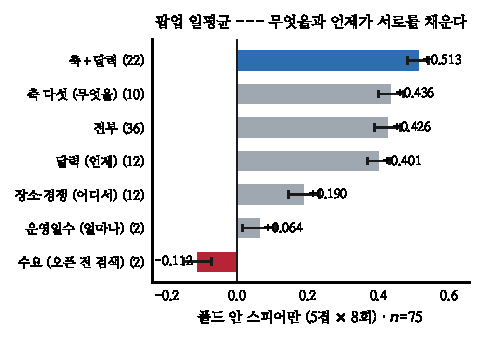
\includegraphics[width=\columnwidth]{figs/blocks.pdf}
\caption{팝업 일평균 예측력을 묶음별로. 괄호는 열 수, 수염은 표준오차.
축과 달력을 합친 것이 각각보다 높다.}
\end{figure}

\section{제품 질문을 잴 수 있는 형태로}

노트 130은 팝업 일평균과 제일 세게 붙는 것이 주말 비중($+$0.427)이고 오픈
전 검색이 꼴찌($+$0.088)라는 것으로 끝났다. 거기서 ``기획에서 바꿀 수 있는
것이 별로 안 남는다''고 읽었는데, 그 읽기에 구멍이 있었다.
\textbf{주말 비중도 기획자가 고른다.} 언제 열지는 기획의 일부다.

그래서 질문을 바꿨다. \emph{예측 가능한 부분이 어느 묶음에서 오나, 그리고
그 묶음을 기획자가 고를 수 있나.}

\begin{table}[t]
\centering\tsize
\caption{팝업 일평균 · $n$=75 · 5겹 $\times$ 8회, 폴드 안에서 재고 평균.
전부 오픈 이전에 알 수 있는 값이다.}
\begin{tabular}{lrrl}
\toprule
& 열 & $\rho$ & \\
\midrule
\textbf{축 $+$ 달력} & 22 & \textbf{$+$.513} & 통제 가능 \\
축 다섯 (무엇을) & 10 & $+$.436 & 통제 가능 \\
달력 (언제) & 12 & $+$.401 & 통제 가능 \\
전부 & 36 & $+$.426 & \\
장소 · 경쟁 (어디서) & 12 & $+$.190 & 통제 가능 \\
운영일수 (얼마나) & 2 & $+$.064 & 통제 가능 \\
오픈 전 검색 (수요) & 2 & $-$.112 & 통제 못 함 \\
\bottomrule
\end{tabular}
\end{table}

\claimx{\textbf{무엇을과 언제가 서로를 채운다.} 각각 $+$0.436과 $+$0.401인데
합치면 $+$0.513이다. 겹치는 정보가 아니라 다른 정보다.}{표준오차가
0.030$\sim$0.047이다. $+$0.513과 $+$0.436의 차이는 두 표준오차쯤이라
갈리지만, $+$0.436과 $+$0.401 사이는 안 갈린다.}

\claimx{\textbf{더 넣으면 내린다.} 축 $+$ 달력이 22열에 $+$0.513인데 장소 ·
경쟁 · 운영일수까지 36열로 늘리면 $+$0.426이다. $n$=75에 36열은 너무
많다.}{그 두 묶음이 쓸모없다는 뜻은 아니다 --- 표본이 늘면 달라질 수 있다.
지금 표본에서 쓰면 손해라는 것이다.}

\claimx{\textbf{그리고 오픈 전 검색은 팝업에서 해롭다}($-$0.112). 노트
128부터 세 노트에 걸쳐 팝업만 검색 축의 덕을 못 본다고 적었는데, 이제
``덕을 못 본다''가 아니라 \emph{음수}로 확정된다.}{팝업 검색어가
브랜드명이라서일 수 있다(노트 129). 팝업 이름으로 다시 긁어 보면 갈리는데,
팝업 이름은 오픈 이전에 검색되지 않는 경우가 많아 창이 빈다.}

\section{그 답을 내는 길에 채점이 틀렸다}

처음 계산에서 이상한 것이 나왔다. 운영일수는 라벨과의 원상관이 $+$0.114인데
교차검증이 $-$0.400으로 나왔다. 부호가 뒤집히는 것은 계산이 틀렸다는 뜻이다.

\begin{figure*}[t]
\centering
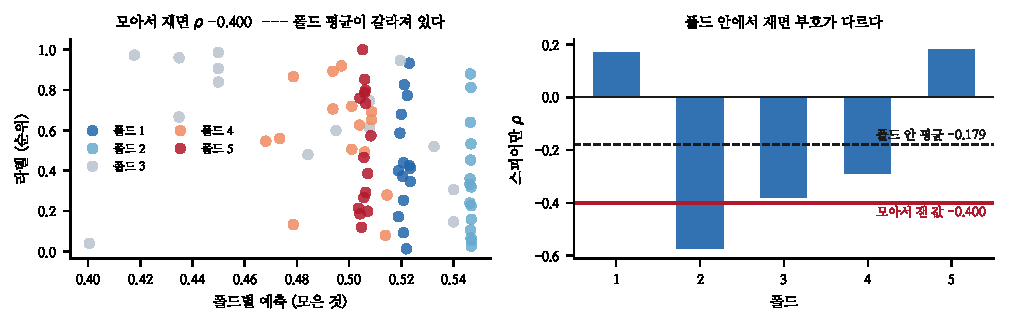
\includegraphics[width=\textwidth]{figs/fold.pdf}
\caption{왼쪽 --- 폴드마다 예측이 좁은 띠에 뭉치고 띠의 위치가 다르다.
모아서 재면 그 띠 사이 간격을 잰다. 오른쪽 --- 폴드 안에서 재면 부호가
갈린다.}
\end{figure*}

\claimx{\textbf{능형이 계수를 0으로 수축시키면 예측이 폴드 평균이 된다.}
폴드별 기울기가 $+$0.005 · $-$0.001 · $+$0.161 · $+$0.049 · $+$0.005로
거의 0이었다. 그러면 각 폴드의 예측은 그 폴드 훈련 평균에 가깝고, 폴드별
예측을 \emph{모아서} 스피어만을 재면 신호가 아니라 \textbf{폴드 간 평균
차이}를 잰다. 라벨을 전체에서 순위화해 놓았으니 그 차이가 라벨과 우연히
정렬돼 $-$0.400이 나왔다.}{폴드 안에서 재도 한 분할만 쓰면 폴드당 15건이라
잡음이 크다($-$0.57$\sim$$+$0.19). 8회 반복해 평균해야 $+$0.064로 안정된다.}

노트 127의 묶음 결함과 같은 계열이다 --- 예측이 구별을 못 하는데 스피어만은
숫자를 내놓는다. 다만 묶음 가드는 값이 \emph{완전히} 같을 때만 잡으니
``조금씩만 다른'' 이 경우를 놓쳤다.

\claimx{\textbf{그래서 평탄 가드를 걸었다.} 예측 사분위폭이 라벨 사분위폭의
2\%도 안 되면 실패로 적는다. 상시 가드가 여덟이 됐다.}{2\%는 손으로 정한
문턱이다. 이 판에서 정상 실행은 0.64$\sim$0.91이라 여유가 크지만, 경계
근처 사례를 아직 못 봤다.}

\section{웹툰을 채웠다}

노트 129에서 웹툰 덮음이 37.9\%에서 할당량 소진으로 멈춰 있었다. 채웠다.

\begin{table}[t]
\centering\tsize
\caption{검색 축 덮음. 합계 5{,}925행.}
\begin{tabular}{lrr}
\toprule
& 덮음 & \\
\midrule
웹툰 & \textbf{97.6\%} & 37.9\%에서 \\
팝업 & 89.3\% & \\
도서 & 88.5\% & \\
펀딩 & 86.3\% & \\
애니 & 74.6\% & \\
모바일 & 41.3\% & 제목 언어 한계 \\
아이돌 & 34.6\% & \\
게임 & 30.5\% & 제목 언어 한계 \\
만화 · 세계애니 & 0\% & 로마자 제목 \\
\bottomrule
\end{tabular}
\end{table}

\begin{table}[t]
\centering\tsize
\caption{부스팅의 사다리. 축을 더하거나 덮음을 채울 때마다 셋이 같이
좋아진다.}
\begin{tabular}{lrrr}
\toprule
& 판 $\rho$ & 귀무 폭 & $z$ \\
\midrule
공통 다섯 & $+$.3363 & .0789 & $+$4.41 \\
$+$검색 (웹툰 38\%) & $+$.4107 & .0630 & $+$6.57 \\
$+$검색 $+$달력 (38\%) & $+$.4203 & .0579 & $+$7.31 \\
$+$검색 $+$달력 (98\%) & \textbf{$+$.4328} & --- & --- \\
\bottomrule
\end{tabular}
\end{table}

공통 다섯 축만 쓰던 자리에서 총 $+$0.0965다. 노트 125부터 127까지 정식화를
일곱 붙여 얻은 최대 폭이 $+$0.013이었다.

\section{TabPFN --- 모수를 우리 자료로 안 정하는 것}

지시에 있던 ``프론티어급 프로덕트 참고''를 실제로 붙였다. TabPFN은 합성
표 자료 수백만 개로 사전학습된 트랜스포머로, 학습 표를 문맥에 넣고 한 번
통과시켜 예측한다 --- 하이퍼모수도 없고 적합도 없다.

이 판에서 볼 만한 이유가 있다. 노트 126의 법칙은 ``한 도메인의 이력만으로
정해지는 모수는 지평 너머에서 배신한다''였다. TabPFN은 \emph{모수를 우리
자료로 정하지 않는다.} 그렇다면 그 법칙에 안 걸려야 한다.

\claimx{\textbf{조정 없이 손으로 만든 것과 같은 자리에 온다.} 공통 다섯
축에서 판 $\rho$ $+$0.3443이고, F6 직접 풀링 $+$0.3413 · F9 짝 순위
$+$0.3464 사이다. 노트 116까지 축 스물세 개를 손으로 시험하고 노트 125부터
정식화 일곱을 붙여 얻은 자리를, 이 모형은 코드 서른 줄로 온다.}{8.x는
라이선스 토큰이 필요해 가중치가 공개된 2.2.1을 썼다. 예측이 대상당 150초로
느려서 가드 전부를 붙이기에는 아직 비싸다 --- 문맥을 3{,}000행으로 잘랐다.}

\section{남은 것}

\begin{table}[t]
\centering\tsize
\caption{다음.}
\begin{tabular}{ll}
\toprule
TabPFN & 축을 주면 같이 오르나 (도는 중) \\
달력 & 왜 트리에서만 되나 --- 계수 방향 일치가 부분 근거 \\
모바일 · 게임 & 제목 언어로 덮음이 30$\sim$41\%에 묶여 있다 \\
팝업 & 무엇을 $+$ 언제로 좁힌 모형을 배포 규약에서 재기 \\
\bottomrule
\end{tabular}
\end{table}

달력이 왜 부스팅에서만 값을 하는지에 부분 근거를 하나 얻었다. 도메인마다
달력 계수 벡터를 맞추고 쌍 코사인을 재면 평균 $+$0.198인데, 검색 축은
$+$0.331이다. 검색은 방향까지 공유하고 달력은 덜 공유한다 --- 트리는
도메인 표시자로 쪼갤 수 있으니 그 차이를 흡수한다. \textbf{다만 이것도
정황이다} --- 도메인이 7$\sim$10개뿐이고 범위가 $-$0.76에서 $+$0.96까지
넓다.

\end{document}
